\documentclass[11pt]{article}

\newcommand{\yourname}{}
\newcommand{\yourcollaborators}{}

\def\comments{0}

%format and packages%\usepackage{algorithm, algorithmic}
\usepackage{algpseudocode}
\usepackage{amsmath, amssymb, amsthm}
\usepackage{enumerate}
\usepackage{enumitem}
\usepackage{framed}
\usepackage{verbatim}
\usepackage[margin=1.0in]{geometry}
\usepackage{multirow}

\usepackage{microtype}


\usepackage{graphicx}
\usepackage{tikz}
\usetikzlibrary{automata, positioning, arrows.meta}

	\definecolor{processblue}{cmyk}{0.96,0,0,0}


\usepackage{kpfonts}
\usepackage{palatino}
	\DeclareMathAlphabet{\mathtt}{OT1}{cmtt}{m}{n}
	\SetMathAlphabet{\mathtt}{bold}{OT1}{cmtt}{bx}{n}
	\DeclareMathAlphabet{\mathsf}{OT1}{cmss}{m}{n}
	\SetMathAlphabet{\mathsf}{bold}{OT1}{cmss}{bx}{n}
	\renewcommand*\ttdefault{cmtt}
	\renewcommand*\sfdefault{cmss}
	\renewcommand{\baselinestretch}{1.06}
\usepackage{tikz}
	\usetikzlibrary{positioning}
	\definecolor{processblue}{cmyk}{0.96,0,0,0}
    \usetikzlibrary{matrix,arrows}

\tikzset{
->, % makes the edges directed
>=Stealth, % makes the arrow heads bold
node distance=3cm, % specifies the minimum distance between two nodes. Change if necessary.
every state/.style={thick, fill=gray!10}, % sets the properties for each ’state’ node
initial text=$ $, % sets the text that appears on the start arrow
}
	
\usepackage{hyperref}

\hypersetup{
	linktocpage=true,
	colorlinks=true,				% false: boxed links; true: colored links
	linkcolor=blue,		% color of internal links
	citecolor=blue,	% color of links to bibliography
	urlcolor=blue,		% color of external links
}

\usepackage[boxruled,vlined,nofillcomment]{algorithm2e}
	\SetKwProg{Fn}{Function}{\string:}{}
	\SetKwFor{While}{While}{}{}
	\SetKwFor{For}{For}{}{}
	\SetKwIF{If}{ElseIf}{Else}{If}{:}{ElseIf}{Else}{:}
	\SetKw{Return}{Return}

%enclosure macros
\newcommand{\paren}[1]{\ensuremath{\left( {#1} \right)}}
\newcommand{\bracket}[1]{\ensuremath{\left\{ {#1} \right\}}}
\renewcommand{\sb}[1]{\ensuremath{\left[ {#1} \right\]}}
\newcommand{\ab}[1]{\ensuremath{\left\langle {#1} \right\rangle}}

%probability macros
\newcommand{\ex}[2]{{\ifx&#1& \mathbb{E} \else \underset{#1}{\mathbb{E}} \fi \left[#2\right]}}
\newcommand{\pr}[2]{{\ifx&#1& \mathbb{P} \else \underset{#1}{\mathbb{P}} \fi \left[#2\right]}}
\newcommand{\var}[2]{{\ifx&#1& \mathrm{Var} \else \underset{#1}{\mathrm{Var}} \fi \left[#2\right]}}

%useful CS macros
\newcommand{\poly}{\mathrm{poly}}
\newcommand{\polylog}{\mathrm{polylog}}
\newcommand{\zo}{\{0,1\}}
\newcommand{\pmo}{\{\pm1\}}
\newcommand{\getsr}{\gets_{\mbox{\tiny R}}}
\newcommand{\card}[1]{\left| #1 \right|}
\newcommand{\set}[1]{\left\{#1\right\}}
\newcommand{\negl}{\mathrm{negl}}
\newcommand{\eps}{\varepsilon}
\DeclareMathOperator*{\argmin}{arg\,min}
\DeclareMathOperator*{\argmax}{arg\,max}
\newcommand{\eqand}{\qquad \textrm{and} \qquad}
\newcommand{\ind}[1]{\mathbb{I}\{#1\}}
\newcommand{\sslash}{\ensuremath{\mathbin{/\mkern-3mu/}}}

%mathbb
\newcommand{\N}{\mathbb{N}}
\newcommand{\R}{\mathbb{R}}
\newcommand{\Z}{\mathbb{Z}}
%mathcal
\newcommand{\cA}{\mathcal{A}}
\newcommand{\cB}{\mathcal{B}}
\newcommand{\cC}{\mathcal{C}}
\newcommand{\cD}{\mathcal{D}}
\newcommand{\cE}{\mathcal{E}}
\newcommand{\cF}{\mathcal{F}}
\newcommand{\cL}{\mathcal{L}}
\newcommand{\cM}{\mathcal{M}}
\newcommand{\cO}{\mathcal{O}}
\newcommand{\cP}{\mathcal{P}}
\newcommand{\cQ}{\mathcal{Q}}
\newcommand{\cR}{\mathcal{R}}
\newcommand{\cS}{\mathcal{S}}
\newcommand{\cU}{\mathcal{U}}
\newcommand{\cV}{\mathcal{V}}
\newcommand{\cW}{\mathcal{W}}
\newcommand{\cX}{\mathcal{X}}
\newcommand{\cY}{\mathcal{Y}}
\newcommand{\cZ}{\mathcal{Z}}

\newcommand{\opt}{\textsc{opt}}

%theorem macros
\newtheorem{thm}{Theorem}
\newtheorem{lem}[thm]{Lemma}
\newtheorem{fact}[thm]{Fact}
\newtheorem{clm}[thm]{Claim}
\newtheorem{rem}[thm]{Remark}
\newtheorem{coro}[thm]{Corollary}
\newtheorem{prop}[thm]{Proposition}
\newtheorem{conj}[thm]{Conjecture}

\theoremstyle{definition}
\newtheorem{defn}[thm]{Definition}


\newcommand{\instructor}{Drew van der Poel}
\newcommand{\hwnum}{6}
\newcommand{\hwdue}{Friday, August 19 at 11:59pm via \href{https://www.gradescope.com/courses/406943}{Gradescope}}

\theoremstyle{theorem}
\newtheorem{prob}{Problem}
\newtheorem{sol}{Solution}

\definecolor{cit}{rgb}{0.05,0.2,0.45} 
\newcommand{\solution}{\medskip\noindent{\color{blue}\textbf{Solution:}}}

\begin{document}
{\Large 
\begin{center}{CS3800: Theory of Computation} --- Summer II '22 --- \instructor \end{center}}
{\large
\vspace{10pt}
\noindent Homework~\hwnum \vspace{2pt}\\
Due~\hwdue}

\bigskip
{\large
\noindent Name: \yourname \vspace{2pt}\\ Collaborators: \yourcollaborators}

\vspace{15pt}
\begin{itemize}

\item Make sure to put your name on the first page.  If you are using the \LaTeX~template we provided, then you can make sure it appears by filling in the \texttt{yourname} command.

\item This assignment is due~\hwdue.  No late assignments will be accepted.  Make sure to submit something before the deadline.

\item Solutions must be typeset.  If you need to draw any diagrams, you may draw them by hand as long as they are embedded in the PDF.  I recommend using the source file for this assignment to get started.

\item I encourage you to work with your classmates on the homework problems. \emph{If you do collaborate, you must write all solutions by yourself, in your own words.}  Do not submit anything you cannot explain.  Please list all your collaborators in your solution for each problem by filling in the \texttt{yourcollaborators} command.

\item Finding solutions to homework problems on the web, or by asking students not enrolled in the class is strictly forbidden.

\end{itemize}


\newpage

\begin{prob} Big-O (\emph{3 points})\end{prob}

For each of the following statements, state whether it is true or false. If it is true, provide an argument as to why (this doesn't have to be overly formal). If it is false, provide a counterexample. 

Note the formal definition of Big-O is as follows: $f(n) =O(g(n))$ if there exist $n_0, c > 0$ such that $f(n) \leq c*g(n)$ for all $n \geq n_0$.

We assume that all functions are positive, continuous, non-decreasing and that they are of the form $\mathbb{N} \rightarrow \mathbb{R}$.

\begin{enumerate}[label=(\alph*)]


\item \textbf{[1 pt.]} For any pair of functions $f(n)$ and $g(n)$, either $f(n) + g(n) = O(f(n))$ or $f(n) + g(n) = O(g(n))$.

\solution\\
True, you can break $f(n)$ and $g(n)$ into 3 cases: \\~\\

$f(n) > g(n)$ \hspace{0.5cm} $\forall n \geq n_0$:\\~\\
In this case,  $f(n) + g(n) = O(f(n)) $  



\item \textbf{[1 pt.]} For any pair of functions $f(n)$ and $g(n)$, if $f(n) + g(n) = O(f(n))$ then $f(n) > g(n)$ for all $n \geq n_0$.

\solution

False, if we let $f(n) = n$ and $g(n) = n$ then $f(n) + g(n) = 2n$\\~\\
$f(n) + g(n) \leq c * f(n)$ \hspace{0.4cm} $\forall n \geq n_0$  \\~\\ 
$2n \leq c * n$  \\~\\
This is true if $c = 2$ and $n_0 = 1$ \\~\\
Therefore, $f(n) + g(n) = O(f(n))$ but $f(n) = g(n)$ for all $n \geq n_0$



\item \textbf{[1 pt.]} For any pair of functions $f(n)$ and $g(n)$, if $f(n) + g(n) = O(f(n))$ and $f(n) + g(n) = O(g(n))$, then $f(n) = g(n)$.

\solution \\
False, if we let $f(n) = n$ and $g(n) = 2n$ then $f(n) + g(n) = 3n$: \\~\\
1a. $f(n) + g(n) \leq c * f(n)$ \hspace{0.4cm} $\forall n \geq n_0$  \\
1b. $3n \leq c * n$ \hspace{0.4cm} \\ 
1c. This is true if $c = 3$ and $n_0 = 1$ \\
Therefore, $f(n) + g(n) = O(f(n))$ \\~\\
2a. $f(n) + g(n) \leq c * g(n)$ \hspace{0.4cm} $\forall n \geq n_0'$  \\
2b. $3n \leq c * 2n$ \hspace{0.4cm} \\ 
2c. This is true if $c = 1.5$ and $n_0' = 1$ \\
Therefore, $f(n) + g(n) = O(g(n))$ \\~\\
$f(n) + g(n) = O(f(n))$ and  $f(n) + g(n) = O(g(n))$ but $f(n) \neq g(n)$






\end{enumerate}


\newpage

\begin{prob} 7th-Smallest is P (\emph{4 points})\end{prob}

Consider the following problem \textsc{7th-Smallest}. You are given an array containing $n>100$ natural numbers and are tasked with finding the 7th smallest value. Show that \textsc{7th-Smallest} $\in P$. State the running time of your algorithm on a deterministic single-tape Turing machine in terms of the length of the input array on the tape. You can use any reasonable encoding, just be sure to state the encoding and what the length of the input array is.

\solution\\
Let $M$ be the Turing Machine that decides \textsc{7th-Smallest} where the input to $M$ is $<A>$, the encoding of the input array. \\~\\
The input array will use a unary encoding for each number with a $*$ delimiter separating each number in the array. Let $n$ be the length of the input array and let $L$ be the length of the string encoding for the largest number in $A$, then the length of the encoding, $\langle A \rangle$, is: \\
$O(nL)$ \\~\\
TM $M$ = On input $\langle A \rangle$: \\
\hspace*{0.5cm}
\begin{minipage}{.87\textwidth}
	while
\end{minipage}


\newpage

\begin{prob} Reduction Practice (\emph{7 points})\end{prob}

Consider the following two problems:\\

\textsc{DirectedHamiltonianCycle} $= \{ \langle G \rangle | \text{ directed graph G contains a directed Hamiltonian cycle} \}$

\textsc{UndirectedHamiltonianCycle} $= \{ \langle G \rangle | \text{ undirected graph G contains a Hamiltonian cycle} \}$\\

Note that a (directed) Hamiltonian cycle is a simple (directed) cycle, which visits every node in the graph exactly once. Recall that a simple cycle means that no vertex or edge repeats (except for the first/last node).

Show that \textsc{DirectedHamiltonianCycle} is mapping reducible to \textsc{UndirectedHamiltonianCycle}. Show why your reduction works on the following graph (which has no directed Hamiltonian cycle) by applying your reduction and arguing why the resulting graph has no undirected Hamiltonian cycle:

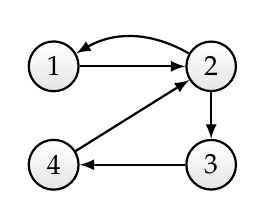
\begin{tikzpicture}[>= latex,node distance = 1.25 cm and 2.0cm,on grid, thick,state/.style ={circle,top color =white,bottom color = gray!20,draw,black,text=black,minimum width =.2 cm}]
\node[state] (a) {1};
\node[state] (b) [right =of a] {2};
\node[state] (c) [below =of b] {3};
\node[state] (d) [below =of a] {4};

\path[->] 	(a) edge node {} (b)
				(b) edge node {} (c)
(c) edge node {} (d)
(d) edge node {} (b);
\path[->]	(b) edge[bend right]  node {} (a);
\end{tikzpicture}


\solution




\newpage

\begin{prob} Thought Experiment (\emph{6 points})\end{prob}


\begin{enumerate}[label=(\alph*)]

\item \textbf{[2 pts.]} Recall $E_{TM}$, the Turing machine emptiness problem, and the $\overline{EQ_{TM}}$, the complement of the Turing machine equivalence problem. We know $E_{TM}$ is undecidable. Use a general reducibilty argument to show that $\overline{EQ_{TM}}$ is undecidable.

\solution \\
Assume true that $\overline{EQ_{TM}}$ is decidable, so there exists a Turing Machine, $D$, that decides $\overline{EQ_{TM}}$. \\~\\
Let $S$ be a Turing Machine that takes in the same inputs as the $E_{TM}$ problem, $\langle M\rangle$ where $M$ is some TM. \\~\\
TM $S =$ on input $\langle M \rangle$: \\~\\
\hspace*{0.54cm}
\begin{minipage}{0.9\textwidth}
	1. Construct a new Turing Machine, $B$ that takes in an arbitrary string $\langle x \rangle$\\~\\
	TM $B$ = on input $\langle x \rangle$: \\~\\
	\hspace*{0.9cm}
	\begin{minipage}{1.2\textwidth}
		a. $B$ rejects $x$\\
	\end{minipage}
	(So $L(B) = \varnothing$) \\~\\
	2. Run $D$ on $\langle M, B \rangle$, if $D$ rejects by halting then $S$ should accept \\
	else if $D$ accepts then $S$ should reject\\~\\
\end{minipage}

Therefore, with the help of $D$, the TM that decides $\overline{EQ_{TM}}$, there exists a TM $S$ that decides $E_{TM}$ which is a contradiction since $E_{TM}$ is undecidable. Hence, TM $D$ cannot exist which means that $\overline{EQ_{TM}}$ is undecidable.



\item \textbf{[2 pts.]}  We said in class that just because we are able to use a general reducibility argument to show undecidability, doesn't mean that that argument can be extended to show unrecognizabiility. We will show an example of such a case with attempting to extend the reduction from part (a). Note that we showed in class that $E_{TM}$ is unrecognizable. 

Suppose we try to make an unrecognizability argument by reducing $E_{TM}$ to $\overline{EQ_{TM}}$.
What is our initial assumption? What does this imply about the existence of a Turing machine? What is the input and behavior of this machine?

\solution \\
We assume that $\overline{EQ_{TM}}$ is recognizable, so this implies the existence of a Turing Machine, $D$, that recognizes $\overline{EQ_{TM}}$. The input to $D$ would be $\langle M_1, M_2 \rangle$ where $M_1$ and $M_2$ are Turing Machines.


\item \textbf{[1 pt.]} Now we want to work towards a contradiction. Given that we are reducing from $E_{TM}$, what is the contradiction we'd like to arrive at? What exactly would we need to show exists?

\solution \\
We need to show that with the existence of $D$, we can construct a Turing Machine, $S$, that recognizes $E_{TM}$. This is the contradiction we would like to arrive at since we know $E_{TM}$ is unrecognizable and therefore, $S$, cannot exist. 



\item \textbf{[1 pt.]} Given what we are assuming in part (b) and what we'd like to show in part (c), explain why we aren't able to use our Turing machine from part (b) to complete the necessary task in part (c). 

\solution





\end{enumerate}

\newpage

\begin{prob} Fun with Encodings (\emph{10 points})\end{prob}

Consider a Turing machine which takes as input a natural number $x$ and repeatedly decrements $x$ (sets $x=x-1$) until $x=0$. 

We use this simple process to illustrate the impact that the string encoding has on the runtime. To further highlight the differences, we require that when going from $x$ to $0$, the Turing machine goes through a series of checkpoints where only $\langle x \rangle$ is on the tape, then only $\langle x-1 \rangle$ is on the tape, and so on until only $\langle 1 \rangle$ is on the tape, and finally only $\langle 0 \rangle$ is on the tape. Note that other strings may be on the tape in between $\langle i \rangle$ and $\langle i-1 \rangle$, we just need to ensure that each checkpoint is hit.

\begin{enumerate}[label=(\alph*)]

\item \textbf{[2 pts.]} First consider using a unary encoding. That is, if $x = 5$, $\langle x \rangle = 11111$. We'll assume $x=0$ is represented by a blank tape. Give an algorithm which follows the checkpoints as stated above. Analyze the running time in terms of (1) the length of the encoding of $x$ ($|\langle x \rangle|$) and (2) the value of $x$ ($x$).

\solution\\
Let $M$ be the TM on this process, on input $\langle x \rangle$: \\~\\
\hspace*{0.5cm}
\begin{minipage}{0.9\textwidth}
1. move right until we've found the last 1 on the tape   \\~\\
2. while we're currently on a 1: \\~\\
\hspace*{0.54cm}
\begin{minipage}{0.9\textwidth}
	a. replace the 1 with a $\sqcup$ (empty cell) and move to the left by one \\
\end{minipage}
3. if we're currently on a $\sqcup$, $M$ will halt on an accept state  
\end{minipage}


\item \textbf{[2 pts.]} Now we update the notion of a checkpoint to enforce that the tape head is in the first (leftmost) cell when the encoding of each value is on the tape.
Give an algorithm which follows this new notion of checkpoint. Analyze the running time in terms of (1) the length of the encoding of $x$ and (2) the value of $x$.

\solution \\
Let $M$ be the TM on this new process, on input $\langle x \rangle$: \\~\\
\hspace*{0.5cm}
\begin{minipage}{0.9\textwidth}
1. while we're currently on a 1: \\~\\
\hspace*{0.54cm}
\begin{minipage}{0.9\textwidth}
	a. mark our current cell as $1$* \\
	b. move right until we've found the last 1 \\
	c. if we're currently on a 1 or $1$*, replace it with a $\sqcup$ (empty cell) \\
	d. move left once \\
	e. move left until we've at a $1$* or $\sqcup$ \\
	f. if we're at a $1$* replace it with 1 \\
\end{minipage}
3. if we're currently on a $\sqcup$, $M$ will halt on an accept state    
\end{minipage}


\item \textbf{[4 pts.]} Now we consider a binary encoding. That is, if $x = 5$, $\langle x \rangle = 101$.
Give an algorithm which follows the original notion of checkpoint used in part (a). Analyze the running time in terms of (1) the length of the encoding of $x$ and (2) the value of $x$.

\solution \\
Let $M$ be the TM on this process, on input $\langle x \rangle$: \\~\\
\hspace*{0.5cm}
\begin{minipage}{0.9\textwidth}
1. if we're currently on a 1 or 0: \\~\\
\hspace*{0.6cm}
\begin{minipage}{1.2\textwidth}
	  a. mark the start as 1* \\
	  b. move right until we've found the last 1 or 0 on the tape \\
	  c. if we are on a 1, replace it with a 0\\
	  d. else if we are on 1*: replace it with $\sqcup$\\
	  e. else if we are on 0: \\~\\
	  \hspace*{0.37cm}
	  \begin{minipage}{1.1\textwidth}
		i. move left until we find the next 1 or 1*: \\~\\
		\hspace*{0.7cm}
		\begin{minipage}{1.2\textwidth}
			while we are moving left, replace 0's with 1's \\
		\end{minipage}
		ii. if we've found a 1, replace it with a 0 \\
		iii. else if we've found a 1*, replace it with 0* \\
		iv. else if we can't find anymore 1's or 1*'s, move right and replace all 0's, 1's and 0*'s with $\sqcup$\\
		and proceed to step 3  \\
	  \end{minipage}
	  f. move left until we've found a 1* or 0*: \\~\\
	\hspace*{0.6cm}
	\begin{minipage}{1.2\textwidth}
		i. if we've found a 1*, replace it with 1 \\
		ii. if we've found a 0*, replace it with $\sqcup$ and shift all of the 1s and 0s to the left by 1 \\
	\end{minipage}
	g. repeat step 1 if condition applies \\~\\
\end{minipage}
2. if we're currently on a $\sqcup$, $M$ will halt on an accept state  
\end{minipage}



\item \textbf{[2 pts.]} State the ordering of the algorithms from parts a, b, and c when measuring runtime in terms of the length of the encoding of $x$. Then state the ordering of the algorithms from parts a, b, and c when measuring runtime in terms of the value of $x$

\solution




\end{enumerate}






\end{document}
